\documentclass[UTF8]{ctexart}
\usepackage[a4paper,left=3cm,right=3cm,top=2cm]{geometry}
\usepackage{amsmath}
\usepackage{enumitem}
\usepackage{float}
\usepackage{threeparttable}
\usepackage{caption}
\usepackage{multirow}
\usepackage{graphicx}
\usepackage{listings}
\usepackage{xcolor}
\renewcommand{\figurename}{Figure}
\definecolor{dkgreen}{rgb}{0,0.6,0}
\definecolor{gray}{rgb}{0.5,0.5,0.5}
\definecolor{mauve}{rgb}{0.58,0,0.82}
\lstset{frame=tb,
  aboveskip=3mm,
  belowskip=3mm,
  showstringspaces=false,
  columns=flexible,
  basicstyle={\small\ttfamily},
  numbers=left,%设置行号位置none不显示行号
  numberstyle=\tiny\courier, %设置行号大小
  numberstyle=\tiny\color{gray},
  keywordstyle=\color{blue},
  commentstyle=\color{dkgreen},
  stringstyle=\color{mauve},
  breaklines=true,
  breakatwhitespace=true,
  escapeinside=`,%逃逸字符(1左面的键),用于显示中文例如在代码中`中文...`
  tabsize=4,
  extendedchars=false %解决代码跨页时,章节标题,页眉等汉字不显示的问题
}

\setlength\lineskiplimit{5.25bp}
\setlength\lineskip{5.25bp}

\title{Lab01 Report}
\author{崔士强 PB22151743}
\date{November 4, 2023}

\bibliographystyle{plain}

\begin{document}

\maketitle
\section{Procedures}
\begin{enumerate}
  \item Load $n$ from the memory.
  \item Determine whether n is odd. If not, flip all bits and add one to get the 2's complement representation of $-n$.
  \item Flip all bits of n. Then we need to count 1.
  \item Multiply $1_{two}$ by $2_{ten}$ to get a number with only one bit 1.
  \item Repeat the process and perform bit-wise AND for 16 times.
  \item If the bit-wise AND operation gives positive number, it means the corresponding bit is 1. Otherwise, it is 0.
  \item Add the last number of Student ID 3 to the result.
  \item Store the results.
\end{enumerate}
\section{Code}
\begin{lstlisting}
  0011 0000 0000 0000       ; starts at memory x3000
  0010 001 011111111        ; load the content of memory x3100 into R1
  0101 010 010 1 00000      ; clear R2
  0101 011 011 1 00000      ; clear R3
  0101 100 100 1 00000      ; clear R4
  0001 100 100 1 01000      ; set R4 as 8
  0001 100 100 1 01000      ; set R4 as 16
  0101 110 110 1 00000      ; clear R6
  0001 010 010 1 00001      ; set R2 as 1
  0101 101 101 1 00000      ; clear R5
  0101 101 001 0 00 010     ; R5 <- R1 AND R2
  0000 001 000000010        ; if not positive, take the 2's complement
  1001 001 001 111111       ; take the negative of R1
  0001 001 001 1 00001      ; R1 plus 1
  1001 001 001 111111       ; NOT R1
  0101 101 001 0 00 010     ; R5 <- R1 AND R2
  0000 010 000000001        ; if zero, the corresponding bit is zero
  0001 011 011 1 00001      ; R3 plus 1
  0001 010 010 0 00 010     ; multiply R2 by 2
  0001 100 100 1 11111      ; R4 substracts 1
  0000 001 111111010        ; if positive, repeat
  0001 110 110 1 00011      ; set R6 as 3
  0001 011 011 0 00 110     ; R3 <- R3 + R6
  0011 110 011101010        ; store the content of R6 into memory x3101
  0011 011 011101010        ; store the content of R3 into memory x3102
  1111 0000 00100101        ; HALT  
\end{lstlisting}
\section{Results}
Test the program 5 times with input respectively 5, 100, 24, 524, 2005. Results are as follows.
\begin{figure}[H]
  \centering
  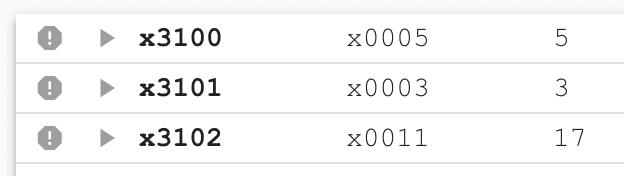
\includegraphics[scale=0.5]{test1.png}
  \caption{Test with 5}
\end{figure}
\begin{figure}[H]
  \centering
  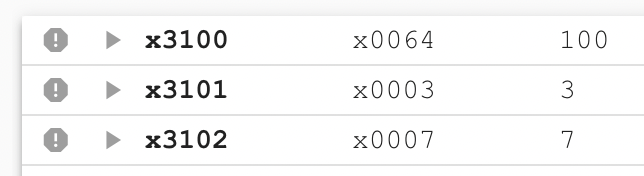
\includegraphics[scale=0.5]{test2.png}
  \caption{Test with 100}
\end{figure}
\begin{figure}[H]
  \centering
  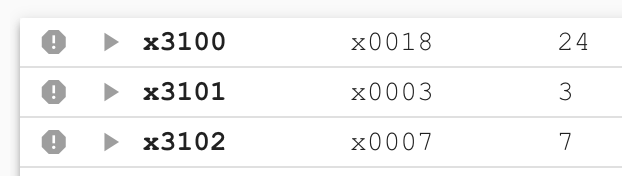
\includegraphics[scale=0.5]{test3.png}
  \caption{Test with 24}
\end{figure}
\begin{figure}[H]
  \centering
  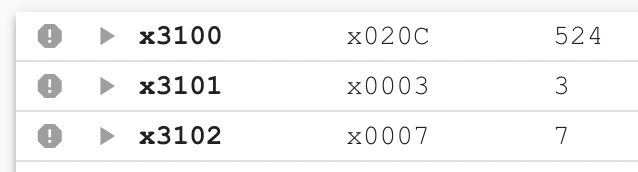
\includegraphics[scale=0.5]{test4.png}
  \caption{Test with 524}
\end{figure}
\begin{figure}[H]
  \centering
  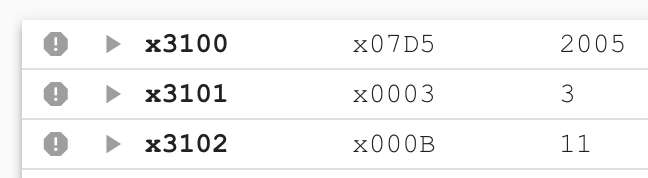
\includegraphics[scale=0.5]{test5.png}
  \caption{Test with 2005}
\end{figure}

All results are correct.
\bibliography{math}

\end{document}
\iffalse
\begin{figure}[h]
    \centering
    \includegraphics[scale=0.5]{name.png}
    \caption{name}
\end{figure}
\fi
